\chapter{Design and Implementation} \label{chap:DesignImplementation}

\section{Overview}\label{sec:Overview}
The basic service \texttt{JMVA} provides is to read in a model definition provided by the user via the \texttt{JMT} front-end, and output performance metrics of the model. This can be a network of \(K\) multiclass servers, with \(R\) classes of customers, and a user-defined population vector \(\mathbf{N}\), which sums to \(N\). These servers may have any one of the following characteristics and inputs:
\begin{itemize}[noitemsep]
    \item \textit{Load-Independent Station}: A demand vector is specified \(\theta_r\) for each class \(r \in [1,R]\).
    \item \textit{Infinite-server/Delay Station}: A delay vector is specified \(\theta_r\) for each class \(r \in [1,R]\).
    \item \textit{Load-Dependent Stations}: A delay matrix is specified \(\theta_{nr}\) for each class \(r \in [1,R]\), and at every possible population load, or queue-length of the station \(n \in N\).
\end{itemize}

The output of the calculation includes, but is not limited to: average station queue lengths \(Q_{kr}\), average throughputs \(\lambda_{r}\), and average response times \(W_{kr}\). For this implementation, the normalizing constant \(G_{\boldsymbol{\theta}}(\mathbf{N})\) is also provided as an output. These evaluation metrics can be calculated via one of the existing queueing network evaluation algorithms (see sections \ref{sec:exact_algos} and \ref{sec:approx_algos}):
\begin{itemize}[noitemsep]
    \item \textit{Exact Algorithms}: Exact Mean-value Analysis (MVA), Method of Moments (MoM), RECAL.
    \item \textit{Approximate Algorithms}: Chow, Bard-Schweitzer and Linearizer algorithms.
\end{itemize}

The implemented software covered in this chapter extends the current JMVA \cite{JavaJMT} suite of tools by introducing a new class of product-form queueing network algorithms: randomized algorithms. In particular, the Logistic Sampling algorithm was implemented, for which the mathematical theory was covered in Chapters \ref{sec:Chapter3} and \ref{sec:Chapter4}. To be exact, the following versions of the Logistic Sampling were implemented:
\begin{itemize}[noitemsep]
    \item \textit{Single-server only networks}: This implementation of the Logistic Sampling algorithm for networks consisting of only \textit{Load-Independent} stations.
    \item \textit{Single-server networks with delay}: This covers \textit{Load-Indepdendent} as well as \textit{Infinite-server/Delay} stations.
    \item \textit{Multi-server networks} This covers \textit{Multi-server} networks (with \(m_i\) servers) with load-dependent demands of the form \(\theta_{nr} = \theta_r/\min(m_i, n)\).
    \item \textit{Multiplicative transform-based logistic sampling}: The version of algorithms for single-server only networks, as well as single server-with-delay networks utilizing the alternative multiplicative transform was implemented, but not available to the front-end.
\end{itemize}

This chapter aims to provide a thorough documentation of the software engineering design choices during the development of these algorithms, implementation details, and how these decisions affect the performance of the implementation. In particular, special attention was paid to the \textit{modularity} of code, as this was an important feature for constant experimentation with new extensions and versions of the above algorithms.
\\\\
We begin by giving an overview of the existing software framework on which the Logistic Sampling package was built on. We then proceed by describing the components of the main \texttt{MonteCarloLogistic} package, which includes the \texttt{Distributions} and \texttt{NumericalIntegration} packages. These provide the required modular tools and classes, required for quick development and testing. The \texttt{Solver} package contains concrete implementations of these classes, for each of the Logistic Sampling algorithms described above.

\section{Existing Architecture}
In this section we outline the general structure and framework in which the software was built on. A more detailed discussion of the general framework is available in \cite{Chugh2012AlgorithmsAnalysis} and \cite{Makaronidis2010EfficientModels}. 
\\\\
At the highest level is the \texttt{analytical} package. All analytical solvers are implemented in the \texttt{analytical.solvers} package, and interfaces with the front end via the \texttt{SolverDispatcher} class. This requires the algorithm to be implemented as a \texttt{Solver} or \texttt{SolverMulti} class. The solver is called in three steps: the Solver is first constructed based on user choice, the model definition is then given as an input to the solver by calling the \texttt{solver.input()} method. \texttt{solver.solve()} is then called by the \texttt{SolverDispatcher} class. The following list covers the sub-packages inside the \texttt{analytical.solvers} framework.
\\\\
{\large \texttt{Control} }\\
This package contains a \texttt{Main} class, which can be run on the command line, in order to bypass the \texttt{JMT} interface. It is responsible for interpreting user input supplied via arguments on the command line. The Logistic Sampling algorithm was added to the available list of algorithms. The implemented algorihms have also been integrated into the \texttt{JMT} frontend.
\\\\
{\large \texttt{DataStructures} }\\
This package contains data structures that are used extensively within the \texttt{analytical} package. These include:
\begin{itemize}
    \item The \texttt{BigRational} class which is a rational fraction of two \texttt{BigIntegers}. Allows for arbitrary-precision numerical calculations. It is used mainly in the \texttt{QNModel} class, in the context of this project.
    \item The \texttt{QNModel} encapsulates the description of a Queueing Network via user model inputs as described in the section \ref{sec:Overview}. It also stores results for performance indices and normalizing constants in the \texttt{BigRational} format.
\end{itemize}

{\large \texttt{QueueingNet} }\\
This is a package that provides a convenient, unified framework for the implementation of newer algorithms in the \texttt{analytical} package. Algorithms are based on the implementation of solvers which extend the \texttt{QNSolver} abstract class, which implements the \texttt{QNSolverInterface} Java interface. The \texttt{QNSolver} abstract class takes in a \texttt{QNModel} object defined in the \texttt{DataStructures} package, and provides a uniform interface to all solvers, allowing easy integration into the package, and re-use of code. The Convolution, CoMoM, and RECAL algorithms are all implemented within this framework.
\\\\
{\large \texttt{Exceptions} }\\
The \texttt{Exceptions} package provides a means for error-handling, and straightforward propagation of meaningful error messages to the front-end. The main class used from this package is the \texttt{InternalErrorExceptions} class. These exceptions can be thrown from within the \texttt{QueueingNet} framework, and is handled by the \texttt{Control} package and \texttt{SolverDispatcher} classes.
\\\\
{\large \texttt{Cern.colt} }\\
The Colt project is a set of Open Source Libraries developed at CERN for high performance scientific computing. It provides a large array of numerical tools, including multidimensional matrix data structures, linear algebra, statistics, common functions, among many others. The main data structures used from this package are the \texttt{DoubleMatrix1D} and \texttt{DoubleMatrix2D} classes which simplifies the implementation of functions defined on multidimensional vector spaces. Tools from the \texttt{random} package was also used in the development of the \texttt{Distributions} package, used in the sampling of multivariate distributions.

\section{The \texttt{Distributions} Package}
The \texttt{Distribution}  package is important as it implements important distributions that are used extensively in the Monte Carlo integration algorithm. This interface enables easy switching and cloning of distributions, allowing for modular re-use of code, as well as scalability. The most important component of this package is the \texttt{MultiVariateRealDistribution} Java Interface.

\subsection*{The \texttt{MultiVariateRealDistribution} Interface}
This interface is designed for use in the \texttt{MCIntegrator} class, and corresponds to a multi-variate distribution over \(\mathbb{R}^K\). This interface requires the following implementation of methods:
\begin{itemize}[noitemsep]
    \item \texttt{getDim()} returns the dimensionality of the multi-variate distribution
    \item \texttt{getSample()} returns a sample in the form of a a \(K\)-dimensional array of the specified distribution.
    \item \texttt{pdf(double[] point)} calculates the pdf of the specified \texttt{point}, or coordinate in the distribution space.
    \item \texttt{copy()} or \texttt{copy(int seed)} provides a method to return an exact copy of the current distribution, or a copy with a different ineteger seed specified. 
\end{itemize}
All distributions implement this interface.

\subsection*{Implementations of \texttt{MultiVariateRealDistribution}}
All implementations of \texttt{MultiVariateRealDistribution} utilize an underlying pseudo-random engine from the \texttt{cern.jet.random} package. The specification of a seed is compulsory when initializing the pseudo-random engine. Across all classes, the seed used is an integer hash of the current datetime obtained via \texttt{java.utils.Date}. The option is also available to the caller to specify an integer seed input given by the user to be added to the datetime seed. This is useful for the definition of multiple instances of the distribution, and ensuring independence. If no integer seed is provided, a default of \texttt{0} is used.
\\\\
The \texttt{ndim}-dimensional \texttt{MultiVariateUniform} distribution is defined by the following constructor:
\begin{lstlisting}
    MultiVariateUniform(int ndim, double[] lb, double[] ub, int seed)
\end{lstlisting}

\texttt{lb} and \texttt{ub} are lower and upper bound arrays of dimensionality \texttt{ndim}.
\\\\
The \texttt{MultiVariateGaussian} is specified with a mean vector array, and a square covariance array:
\begin{lstlisting}
    MultiVariateGaussian(double[] mean, double[][] cov, int seed)
\end{lstlisting}
Underlying the implementation is a \texttt{cern.jet.random.Normal} object which can generate iid Gaussian Samples. The \texttt{cern.colt} \texttt{CholeskyDecomposition} class from their linear algebra package is used to convert the iid Gaussian Samples into one from the specified distribution.
\\\\
The \texttt{MultiVariateStudentT} class, specified via mean and covariance arrays, and a degree-of-freedom, consists of a \texttt{MultiVariateGaussian} and a \texttt{cern.jet.random.ChiSquare} distribution. Together, these distribution can allow one to simulate the correct multivariate student-t distribution:
\begin{lstlisting}
    MultiVariateStudentT(double[] mean, double[][] cov, int df, int seed)
\end{lstlisting}

\section{The \texttt{NumericalIntegration} Package}

\subsection*{The \texttt{Function} Interface}
This interface defines a real, scalar-valued function over a multidimensional domain. The required implementation are as follows:
\begin{itemize}
    \item \texttt{evaluate(double[] point)} : This method is set to return a \texttt{BigDecimal} representing the function value at the specified point
    \item \texttt{copy()}: this method returns a copy of the current function as a \texttt{Function} interface.
\end{itemize}

An abstract class \texttt{SafeFunction} implements this interface by defining 3 new methods:
\begin{itemize}
    \item \texttt{SafeFunction(int ndim)} : The constructor forces the calling procedure to specify a dimensionality \texttt{ndim}.
    \item \texttt{checkPoint(double[] point)} : checks that the dimensionality of the provided evaluation \texttt{point} is correct by checking that its length is equal to its dimensionality.
    \item \texttt{checkInDomain(double[] point)} : abstract method, needs to be implemented by subclass. Allows for the subclass to restrict the evaluation of points to certain conditions.
    \item \texttt{safeEvaluate(double[] point)}: abstract method, implemented by subclass, under the assumption that the \texttt{point} has passed the required safety checks.
\end{itemize}

\begin{lstlisting}[caption= Implementation of \texttt{Function.evaluate()} method by the \texttt{safeFunction} abstract class]
public abstract class SafeFunction implements Function {
    ...
    @Override
    public BigDecimal evaluate(double[] point) throws InternalErrorException {
        this.checkPoint(point);
        this.checkInDomain(point);
        return this.safeEvaluate(point);
    }
}    
\end{lstlisting}

\subsection*{The \texttt{MCIntegrator} class}

The \texttt{MCIntegrator} class implements a multithreaded Monte Carlo Integrator class, specified by providing an instance of a \texttt{Function} interface, a sampling distribution in the form of a \texttt{MultiVariateRealDistribution} instance, the number of samples, and a \texttt{MathContext} instance, which specifies the precision and rounding scheme for BigDecimal operations. The constructor is shown:
\begin{lstlisting}
    MCIntegrator(Function function, MultiVariateRealDistribution dist, int maxnumsamples, MathContext MC, int nthread) 
\end{lstlisting}

Given \texttt{nthread} threads, the \texttt{MCIntegrator} creates \texttt{nthread} instances of a \texttt{SamplingTask} private class. This is an implementation of the \texttt{Callable<V>} interface, where a return type (\texttt{V}) is specified by the implementing class. In this case, \texttt{V} is a \texttt{BigDecimal} return type. All \texttt{Callable} implementations need to implement a \texttt{call()} which computes and returns a result after submission to a thread.
\\\\
A \texttt{SamplingTask} is constructed with a clone of the \texttt{MultiVariateRealDistribution}, \texttt{Function}, and \texttt{MathContext} object from the parent \texttt{MCIntegrator}. The \texttt{seed} variable given to a \texttt{SamplingTask} is the thread number for the particular task, in order to ensure independence of each \texttt{SamplingTask}.
\begin{lstlisting}
    SamplingTask(MultiVariateRealDistribution d, Function f, int n, MathContext MC, int seed)
\end{lstlisting}

During a \texttt{call()} method function call, a \texttt{SamplingTask} generates a number of samples, computes the PDF's of these samples, and performs Monte Carlo Integration using equation (\ref{eq:MCInt}). This is illustrated in the following code listing:
\lstinputlisting[caption=\texttt{SamplingTask} implementation]{Chap5_DesignAndImplementation/SamplingTask.java}

The task is then submitted to a java \texttt{ExecutorService} object and which returns a \texttt{Future<BigDecimal>} object. An instance of a \texttt{Future<V>} object supplies a \texttt{get()} method, which blocks the calling process until \texttt{call() } has finished.

\begin{figure}[H]
\begin{center}
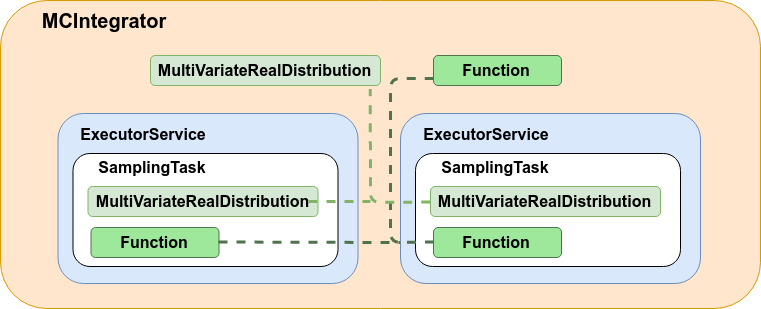
\includegraphics[width=.6\textwidth]{Chap5_DesignAndImplementation/MCIntegrator.png}
\caption{Instance diagram of an 2-thread MCIntegrator object, where the dashed lines denote copies of the same object}
\label{fig:MCIntegrator}
\end{center}
\end{figure}


\section{The \texttt{Solver} Package}
This package encapsulates the core software implementation of the Logistic Sampling algorithm. The classes implemented in this package fall into two main categories, with the exception of the \texttt{MonteCarloLogisticSolver} class which inherits from \texttt{QNSolver}:
\begin{itemize}
    \item Classes inheriting from the \texttt{LogisticFunctionBase} abstract class, which inherits from the \texttt{safeFunction} abstract class, and ultimately from the \texttt{Function} interface. These are implementations of the Integrand functions of the different versions of the Logistic Sampling algorithm. These are summarized in table \ref{table:logistic_function_class_names}. They contain methods to calculate the stationary point an hessian of the stationary point, and get them.
    \item Classes inheriting from the \texttt{LogisticCore} abstract class. \texttt{LogisticCore} is the main class that implements the Logistic Sampling algorithm, with the \texttt{LogisticCoreAdd} and \texttt{LogisticCoreMult} implementing the additive and multiplicative versions of the algorithm.
\end{itemize}

\begin{table}[!htb]
\begin{tabular}{@{}lll@{}}
\toprule
Transform type                  & Function Class Name               & Equation ref. \\ \midrule
\multirow{3}{*}{Additive}       & \texttt{LogisticFunction}         & Single-server network, eq (\ref{eq:log_integrand_single_server}) \\
                                & \texttt{LogisticFunctionDelay}    & Single-server network with delay, eq (\ref{eq:log_integrand_infinite_server})\\
                                & \texttt{LogisticFunctionMS}       & Multi-server network, eq (\ref{eq:log_integrand_multi_server_2})\\
\multirow{2}{*}{Multiplicative} & \texttt{LogisticFunctionMult}     & Single-server network, eq (\ref{eq:log_integrand_single_server_mult})\\
                                &  \texttt{LogisticFunctionMultDelay}  & Single-server network with delay, eq (\ref{eq:log_integrand_infinte_server_mult})\\ \bottomrule
\end{tabular}
\caption{Descriptions of Logistic Function}
\label{table:logistic_function_class_names}
\end{table}

\subsection*{\texttt{LogisticFunctionBase} and subclasses}

\texttt{LogisticFunctionBase} extends the \texttt{safeFunction} abstract class, by adding the following required (abstract) function declarations:
\begin{itemize}[noitemsep]
    \item \texttt{calculate\_stationary\_point}: function to call to calculate (and cache) the stationary point of the specified integrand
    \item \texttt{calculate\_hessian}: function to call to calculate (and cache) the stationary point of the specified integrand
    \item \texttt{getX\_stat}: get stationary point (in transformed domain) of the integrand
    \item \texttt{getHess\_stat}: get stationary point hessian (in transformed domain) of the integrand
\end{itemize}

All integrand functions inherit from \texttt{LogisticFunctionBase} and implement these methods.

Given that the \texttt{LogisticFunction} class inherits from the \texttt{safeFunction} abstract class, it implements its corresponding integrand function in abstract function \texttt{safeEvaluate}. Several design choices were made when implementing the \texttt{LogisticFunction} class, and its related classes:
\begin{itemize}
    \item Cached values include \(\eta_{\epsilon}(N) = N+K(1+\epsilon N)\) and \(\sigma_r = \sum_{k=K}^M \theta_{kr}\) , the latter being only for the \texttt{LogisticFunctionDelay} function. This is to save on a small amount of computation at each sample.
    \item For every class inheriting from the \texttt{LogisticFunctionBase} algorithm, \textit{except for} the \texttt{LogisticFunctionMS} (multiserver) class, the logistic integrand is first computed in terms of its logarithm \(h(\mathbf{x})\), in double precision. This is deemed enough for the logarithm, and has been robustly tested with numerous numerical experiments. The tensor multiplications are performed using the \texttt{DoubleMatrix1D} and \texttt{DoubleMatrix2D} classes from the \texttt{cern.colt} library. The computed log integrand is then raised to \(e^{-h(\mathbf{x})}\) in \texttt{BigDecimal} and returned.
    \item For the \texttt{LogisticFunctionMS} class, all arithmetic operations are performed with \texttt{BigDecimal}, with the specified precision.
    \item For the \texttt{LogisticFunctionMS} class, there is some overhead when enumerating the states and coefficients over which to apply the \(\boldsymbol{\Delta}\) operator in (\ref{eq:log_integrand_multi_server_2}). To save some computation, this is calculated at initialization, and cached. When applying the \(\boldsymbol{\Delta}\) and summation operators, we merely loop over these cached states, multiply by the cached coefficients, and result is summed.
\end{itemize}

For all of the above classes, the precision of the computation of the integrand can be specified by providing a \texttt{MathContext} object to the \texttt{LogisticFunction} class constructor with a specified precision in terms of the number of digits. All \texttt{BigDecimal} operations in the functions are calculated using the specified \texttt{MathContext}.

\subsection*{\texttt{LogisticCore} and subclasses}
The \texttt{LogisticCore} implements the core, higher-level structure of Logistic Sampling algorithm to calculate the normalizing constant, and the logic for distinguishing between the types for models (single-server only, single-server with delay, and multiserver). It is subclassed by the \texttt{LogisticCoreAdd} and \texttt{LogisticCoreMult} classes (for the additive and multiplicative version of the logistic sampling algorithms respectively). Each subclass will implement the \texttt{initialize\_logistic\_function()} which provides the correct version of the logistic function class.
\lstinputlisting[caption=\texttt{LogisticCoreAdd} implementation]{Chap5_DesignAndImplementation/LogisticCoreAdd.java}
\lstinputlisting[caption=\texttt{LogisticCoreMult} implementation]{Chap5_DesignAndImplementation/LogisticCoreMult.java}

\texttt{LogisticCore} then uses these logistic function implementations to calcluate and fetch the stationary point, and the hessian of the integrand at that point. It then finally uses these components to instantiate an \texttt{MCIntegrator} object to perform the integration. This is shown in full in the \texttt{LogisticCore} constructor shown below.
\lstinputlisting[caption=\texttt{LogisticCore} constructor implementation]{Chap5_DesignAndImplementation/LogisticCore.java}

To return the result of the Logistic Sampling algorithm, the public method \texttt{calculateNC()} returns a \texttt{BigDecimal} representing the result of the Monte Carlo Integration.

\subsection*{The Full Solver: \texttt{MonteCarloLogisticSolver}}
In order to provide an interface of the Logistic Core algorithm, the \texttt{MonteCarloLogisticSolver} solver subclass to the \texttt{QNSolver} was written. This class implements the pre-processing of the \texttt{QNModel} input into the solver, by extracting its demand matrix, delays, population vector, and server count. These are then used to check for an invalid model (negative demands, zero total demand for a station etc.). The solver is also responsible for computing and caching the model normalizing constant, and for the calculation of the performance indices (queue lengths and throughputs).
\\\\
To compute the performance indices, the solver has to calculate multiple normalizing constants, as the throughputs and queue lengths are expressed at the ratio of some modified normalizing (\(G'_{\boldsymbol{\theta}}(\mathbf{N})\)) over the true normalizing constant of the model (\(G_{\boldsymbol{\theta}}(\mathbf{N})\)). As a result, the solver instantiates multiple instances of a \texttt{LogisticCore} class, and inputs a modified model. For example the \texttt{augmentDemandsAtServer(int M, int R, DoubleMatrix2D demands, int k)} method is used to augment the model with a specified server \(k\). for the calculation of the queue-lengths at station \(k\).

\lstinputlisting[caption=\texttt{computePerformanceMeasures()} instantiation of multiple \texttt{LogisticCore} instances]{Chap5_DesignAndImplementation/MonteCarloLogisticPerfInd.java}

A full class diagram illustrating the relationships between the classes described above is shown in figure \ref{fig:DistributionsPackage}. 

\newpage
    \begin{figure}[H]
    \begin{center}
    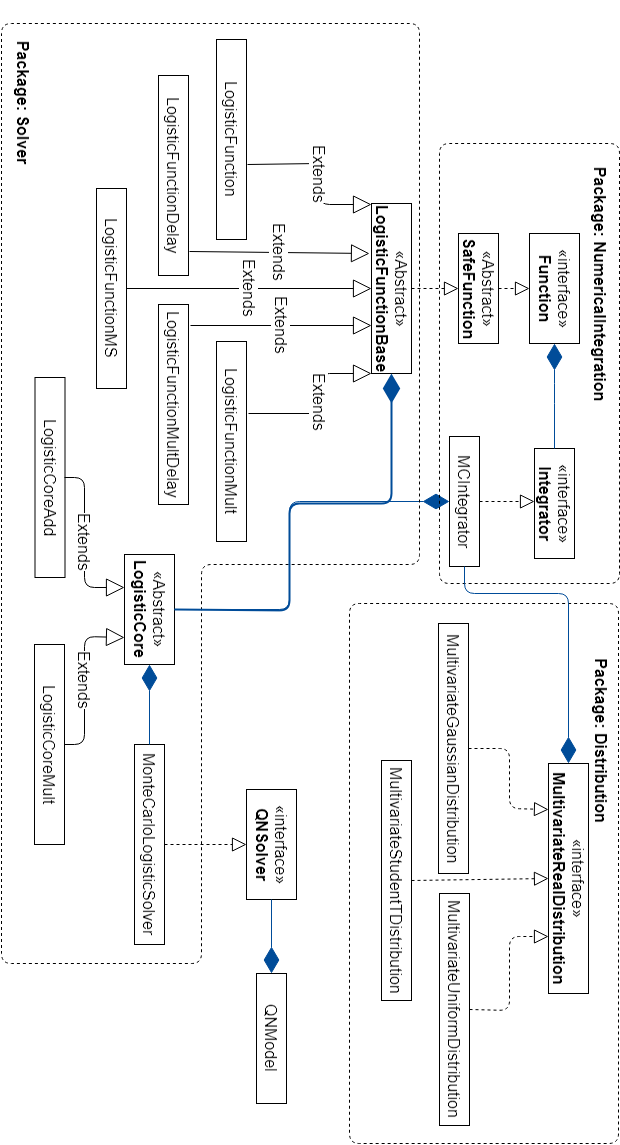
\includegraphics[width=.75\textwidth]{Chap5_DesignAndImplementation/DistributionsPackage.png}
    \caption{Package/class diagram of the implemented components within the \texttt{QueueingNet} framework}
    \label{fig:DistributionsPackage}
    \end{center}
    \end{figure}
\newpage

\section{Testing and Verification}
The modular design of the software has allowed the various components to be tested separately, making it easier to verify correctness for the subcomponents of the Logistic Sampling algorithm. Unit tests were mostly tested against reference implementations written in both MATLAB and python, for related projects, such as \cite{Casale2017AcceleratingMethods}. Unit tests were implemented to cover the following:
\begin{itemize}
    \item Testing the correctness of the implementations of the various distributions in \texttt{Distributions}. Simple example distributions were given, and samples were drawn from the distribution. For example, for the \texttt{MultivariateGaussian} distribution, a simple covariance structure was defined, and samples drawn from the corresponding zero-mean distribution. The maximum-likelihood covariance was computed and verified to be close to the original covariance by taking the matrix 2-norm:
    \[\frac{\Vert \hat{\Sigma}_{ML} - \Sigma \Vert}{\Vert \Sigma \Vert} < \epsilon   \]
    \item Testing the components of \texttt{NumericalIntegration} package. Simple implementations of the \texttt{Function} interface were made and used in conjunction with a simple distribution, in order to test the functionality of \texttt{MCIntegrator}. 
    \item Testing the correctness of the implementations of \texttt{LogisticFunctions} and related classes by checking against reference implementations, given fixed models and input points.
    \item The \texttt{LogisticCore} calculation of the normalizing constant was tested by comparing the log of the normalizing constant against an exact result. For small, simple models, given large enough \(N\), the errors were expected to fall below a reasonable threshold, e.g. \(\epsilon = 0.1\).
\end{itemize}

Ultimately, the true correctness of randomized algorithms can only be verified to a certain degree. The performance of the algorithm was again confirmed through repeated experimentation, which is covered extensively in the following chapters.